%% This is file `elsarticle-template-2-harv.tex',
%%
%% Copyright 2009 Elsevier Ltd
%%
%% This file is part of the 'Elsarticle Bundle'.
%% ---------------------------------------------
%%
%% It may be distributed under the conditions of the LaTeX Project Public
%% License, either version 1.2 of this license or (at your option) any
%% later version.  The latest version of this license is in
%%    http://www.latex-project.org/lppl.txt
%% and version 1.2 or later is part of all distributions of LaTeX
%% version 1999/12/01 or later.222222
%%
%% The list of all files belonging to the 'Elsarticle Bundle' is
%% given in the file `manifest.txt'.
%%
%% Template article for Elsevier's document class `elsarticle'
%% with harvard style bibliographic references
%%
%% $Id: elsarticle-template-2-harv.tex 155 2009-10-08 05:35:05Z rishi $
%% $URL: http://lenova.river-valley.com/svn/elsbst/trunk/elsarticle-template-2-harv.tex $
%%
%%\documentclass[preprint,authoryear,12pt]{elsarticle}

%% Use the option review to obtain double line spacing
%% \documentclass[authoryear,preprint,review,12pt]{elsarticle}

%% Use the options 1p,twocolumn; 3p; 3p,twocolumn; 5p; or 5p,twocolumn
%% for a journal layout:
%% \documentclass[final,authoryear,1p,times]{elsarticle}
%% \documentclass[final,authoryear,1p,times,twocolumn]{elsarticle}
\documentclass[final,authoryear,3p,times]{elsarticle}
%% \documentclass[final,authoryear,3p,times,twocolumn]{elsarticle}
%% \documentclass[final,authoryear,5p,times]{elsarticle}
%% \documentclass[final,authoryear,5p,times,twocolumn]{elsarticle}

%% if you use PostScript figures in your article
%% use the graphics package for simple commands
%% \usepackage{graphics}
%% or use the graphicx package for more complicated commands
%% \usepackage{graphicx}
%% or use the epsfig package if you prefer to use the old commands
%% \usepackage{epsfig}

%% The amssymb package provides various useful mathematical symbols
\usepackage{amssymb}
\usepackage{epstopdf}
\usepackage{lmodern}
\usepackage[latin9]{inputenc}
\usepackage[T1]{fontenc}
\usepackage{color}
\usepackage{float}
\usepackage{tabularx}
\usepackage{breqn}
\usepackage{pgfplots}
\pgfplotsset{compat=1.5}
\newcommand{\mbf}{\mathbf}
%% The amsthm package provides extended theorem environments
%% \usepackage{amsthm}

%% The lineno packages adds line numbers. Start line numbering with
%% \begin{linenumbers}, end it with \end{linenumbers}. Or switch it on
%% for the whole article with \linenumbers after \end{frontmatter}.
%% \usepackage{lineno}

%% natbib.sty is loaded by default. However, natbib options can be
%% provided with \biboptions{...} command. Following options are
%% valid:

%%   round  -  round parentheses are used (default)
%%   square -  square brackets are used   [option]
%%   curly  -  curly braces are used      {option}
%%   angle  -  angle brackets are used    <option>
%%   semicolon  -  multiple citations separated by semi-colon (default)
%%   colon  - same as semicolon, an earlier confusion
%%   comma  -  separated by comma
%%   authoryear - selects author-year citations (default)
%%   numbers-  selects numerical citations
%%   super  -  numerical citations as superscripts
%%   sort   -  sorts multiple citations according to order in ref. list
%%   sort&compress   -  like sort, but also compresses numerical citations
%%   compress - compresses without sorting
%%   longnamesfirst  -  makes first citation full author list
%%
%% \biboptions{longnamesfirst,comma}

% \biboptions{}

\journal{International Journal of Solids and Structures}

%---------------------- editing macros ------------------
\newcommand{\sss}[1]{\textcolor{red}{[\textit{hsp}: #1]}}
\newcommand{\hsp}[1]{\textcolor{blue}{[\textit{ss}: #1]}}
\newcommand{\hspi}[1]{\textcolor{red}{#1}}
\newcommand{\hsps}[1]{\textcolor{red}{\sout{#1}}}
%---------------------- editing macros ------------------

\begin{document}

\begin{frontmatter}

%% Title, authors and addresses

%% use the tnoteref command within \title for footnotes;
%% use the tnotetext command for the associated footnote;
%% use the fnref command within \author or \address for footnotes;
%% use the fntext command for the associated footnote;
%% use the corref command within \author for corresponding author footnotes;
%% use the cortext command for the associated footnote;
%% use the ead command for the email address,
%% and the form \ead[url] for the home page:
%%
%% \title{Title\tnoteref{label1}}
%% \tnotetext[label1]{}
%% \author{Name\corref{cor1}\fnref{label2}}
%% \ead{email address}
%% \ead[url]{home page}
%% \fntext[label2]{}
%% \cortext[cor1]{}
%% \address{Address\fnref{label3}}
%% \fntext[label3]{}

\title{Elastocapillary Effects on Electromechanical Instabilities in Dielectric Elastomers}

%% use optional labels to link authors explicitly to addresses:
%% \author[label1,label2]{<author name>}
%% \address[label1]{<address>}
%% \address[label2]{<address>}

\author[ss]{Saman Seifi}
\ead[ss]{samansei@bu.edu}
\address[ss]{Department of Mechanical Engineering, Boston University, Boston, MA 02215}
\author[hsp]{Harold S. Park}
\ead[hsp]{parkhs@bu.edu}
\address[hsp]{Department of Mechanical Engineering, Boston University, Boston, MA 02215}

\begin{abstract}

We present a new finite deformation, dynamic finite element model that incorporates surface tension to capture elastocapillary effects on the electromechanical deformation of dielectric elastomers.  Single finite element tests with homogeneous and inhomogeneous boundary conditions demonstrate that increasing surface tension results in a larger electric field that is needed to nucleate an electromechanical instability.  We also examine surface tension effects on instabilities in constrained dielectric elastomer films.  In doing so, we find in agreement with recent experimental studies a creasing to wrinkling instability transition as the elastocapillary length increases.  The present results indicate that the proposed methodology may be beneficial in studying the electromechanical deformation and instabilities for dielectric elastomers in the presence of surface tension. 

\end{abstract}

\begin{keyword}
%% keywords here, in the form: keyword \sep keyword
dielectric elastomer \sep elastocapillary
%% MSC codes here, in the form: \MSC code \sep code
%% or \MSC[2008] code \sep code (2000 is the default)

\end{keyword} 

\end{frontmatter}

% \linenumbers

%% main text
\section{Introduction} 

%\footnotetext{\textit{$^{a}$Department of Mechanical Engineering, Boston University, Boston, MA 02215, USA. E-mail:  samansei@bu.edu}}

%\footnotetext{\textit{$^{\ast}$\textit{$^{b}$}~Department of Mechanical Engineering, Boston University, Boston, MA 02215, USA.  Fax:  001 617 353 5866; Tel:  001 617 353 4208; E-mail:  parkhs@bu.edu}}

Dielectric elastomers (DEs) have attracted significant attention in recent years as a soft and flexible actuation material~\citep{carpiSCIENCE2010,brochuMRC2010,biddissMEP2008}.  The salient characteristic of DEs is that if sandwiched between two compliant electrodes that apply voltage across its thickness, the DE can exhibit both significant thinning and in-plane expansion, where the in-plane expansion can often exceed several hundred percent~\citep{keplingerSM2012}.  The ability to undergo such large deformations has led to DEs being studied for both actuation-based applications, including artificial muscles and flexible electronics, and also for generation-based applications and energy harvesting~\citep{carpiSCIENCE2010,brochuMRC2010,mirMT2007}.

Detailed studies on the mechanics of DEs began about 15 years ago with the seminal experimental work of~\citet{pelrineSAA1998,pelrineSCIENCE2000}.  Since then, there have been many experimental~\citep{foxJMPS2008,keplingerPNAS2010,kofodJIMSS2003,kofodSAA2005,peiSPIE2004,planteIJSS2006,planteSAA2007,planteSMS2007,schlaakSPIE2005,wisslerSAA2007a,zhangSPIE2004,chibaSPIE2008,wangPRL2011a,wangAM2012,wangNC2012}, theoretical~\citep{suoJMPS2008,suoAMSS2010,goulbourneJAM2005,dorfmannAM2005,dorfmannJE2006,mcmeekingJAM2005,patrickSAA2007,planteSAA2007,planteSMS2007,wisslerSMS2005}, and recently a small number of computational studies~\citep{parkIJSS2012,parkSM2013,parkCMAME2013,zhouIJSS2008,zhaoAPL2007,vuIJNME2007,wisslerSMS2005,buschelIJNME2013,khanCM2013,henannJMPS2013,liSMS2012} aimed that identifying the mechanisms that have the largest impact on the nonlinear dynamical behavior and failure mechanisms of DEs.  A summary of recent developments on electromechanical instabilities in DEs has been given by~\citet{zhaoAPR2014}.  

Concurrently, researchers have for many years studied the forces exerted by fluids at rest upon solids, which are known as surface tension, or elastocapillary forces.  While the best-known example of surface tension is likely that of deforming liquid droplets, there has been interest in using it to deform solid structures, see the reviews of~\citet{romanJPCM2010} and~\citet{liuAMS2012}.  Specifically, there has recently been interest in using elastocapillary forces to deform \emph{soft} structures in controllable or unique ways, since for these systems the elastocapillary number, which is defined as $\gamma/\mu l$, where $\gamma$ is the surface tension, $\mu$ is the shear modulus and $l$ is a characteristic length, is close to unity, implying that elastocapillary effects can be substantial for these soft materials.  

While elastocapillary effects have been extensively studied in soft materials, its effect on soft materials like DEs that deform when subject to an electric field, is a relatively unknown phenomenon.  For example,~\citet{wangPRE2013} performed interesting experiments of electrostatically deforming a constrained DE in a liquid solution, and showed that the instability mechanism of the surface could be tuned depending on the value of the surface tension.  Furthermore,~\citet{pineiruaSM2010} showed how elastocapillary origami could be developed by coupling surface tension with electric fields to deform a liquid droplet surrounded by a thin sheet of PDMS.  Overall, this discussion makes clear that there may be potential in using surface tension as an additional degree of freedom to introduce new and interesting deformation mechanisms in electroactive polymers like DEs, and furthermore that the computational tools needed to investigate such phenomena are currently lacking.  

Therefore, the objective of the present work is to present a finite element (FE) model for DEs accounting for the effects of surface tension, such that electro-elasto-capillary phenomena in DEs can be computationally investigated.  We pay particular interest to those instances where surface tension couples to and impacts known electromechanical instabilities that dielectric elastomers are known to undergo, specifically snap-through instability~\citep{pelrineSCIENCE2000} and surface creasing and wrinkling~\citep{wangPRL2011,wangAM2012,wangPRE2013}.
ion as an additional degree of freedom to introduce new and interesting deformation mechanisms in electroactive polymers like DEs, and furthermore that the computational tools needed to investigate such phenomena are currently lacking.  

Therefore, the objective of the present work is to present a finite element model for DEs accounting for the effects of surface tension, such that electro-elasto-capillary phenomena in DEs can be computationally investigated.  We pay particular interest to those instances where surface tension couples to and impacts known electromechanical instabilities that dielectric elastomers are known to undergo, specifically snap-through instability~\citep{pelrineSCIENCE2000}, surface creasing~\citep{wangPRL2011,wangAM2012}, and bursting drops leading to crack-like propagation~\citep{wangNC2012}.

\section{Background: Nonlinear Electromechanical Field Theory}

The numerical results we present in this work are based upon a FE discretization of the electromechanical field theory recently proposed by~\citet{suoJMPS2008}, and recently reviewed by~\citet{suoAMSS2010}.   In this field theory at mechanical equilibrium, the nominal stress $S_{iJ}$ satisfies the following (weak) equation:
\begin{equation}\label{eq:suo1} \int_{V}S_{iJ}\frac{\partial\xi_{i}}{\partial X_{J}}dV=\int_{V}\left(B_{i}-\rho\frac{\partial^{2}x_{i}}{\partial t^{2}}\right)\xi_{i}dV+\int_{A}T_{i}\xi_{i}dA,
\end{equation}
where $\xi_{i}$ is an arbitrary vector test function, $B_{i}$ is the body force per unit reference volume $V$, $\rho$ is the mass density of the material and $T_{i}$ is the force per unit area that is applied on the surface $A$ in the reference configuration.  

For the electrostatic problem, the nominal electric displacement $\tilde{D}_{I}$ satisfies the following (weak) equation:
\begin{equation}\label{eq:suo2} -\int_{V}\tilde{D}_{I}\frac{\partial\eta}{\partial X_{I}}dV=\int_{V}q\eta dV+\int_{A}\omega\eta dA,
\end{equation}
where $\eta$ is an arbitrary scalar test function, $q$ is the volumetric charge density and $\omega$ is the surface charge density, both with respect to the reference configuration.  It can be seen that the strong form of the mechanical weak form in (\ref{eq:suo1}) is the momentum equation, while the strong form of the electrostatic weak form in (\ref{eq:suo2}) is Gauss's law.  

As the governing field equations in (\ref{eq:suo1}) and (\ref{eq:suo2}) are decoupled, the electromechanical coupling occurs through the material laws.  The hyperelastic material law we adopt here has been utilized in the literature to study the nonlinear deformations of electrostatically actuated polymers; see the works of~\citet{vuIJNME2007}, and~\citet{zhaoAPL2007}.  Due to the fact that the DE is a rubber-like polymer, phenomenological free energy expressions are typically used to model the deformation of the polymer chains.  In the present work, we will utilize the form~\citep{vuIJNME2007,zhaoAPL2007}
\begin{equation}\label{eq:de1} W(\mbf{C},\tilde{\mbf{E}})=\mu W_{0}-\frac{1}{2}\lambda(\ln{J})^{2}-2\mu W_{0}(3)\ln{J}-\frac{\epsilon}{2}JC_{IJ}^{-1}\tilde{E}_{I}\tilde{E}_{J},
\end{equation}
where $W_{0}$ is the mechanical free energy density in the absence of an electric field, $\epsilon$ is the permittivity, $J=\det(\mbf{F})$, where $\mbf{F}$ is the continuum deformation gradient, $C_{IJ}^{-1}$ are the components of the inverse of the right Cauchy-Green tensor $\mbf{C}$, $\lambda$ is the bulk modulus and $\mu$ is the shear modulus.  

We model the mechanical behavior of the DE using the Arruda-Boyce rubber hyperelastic function~\citep{arrudaJMPS1993}, where the mechanical free energy $W_{0}$ in (\ref{eq:de1}) is approximated by the following truncated series expansion,
\begin{eqnarray}\label{eq:de2} W_{0}(I_{1})=\frac{1}{2}(I_{1}-3)+\frac{1}{20N}(I_{1}^{2}-9)+\frac{11}{1050N^{2}}(I_{1}^{3}-27) \\ \nonumber
+\frac{19}{7000N^{3}}(I_{1}^{4}-81)+\frac{519}{673750N^{4}}(I_{1}^{5}-243),
\end{eqnarray}
where $N$ is a measure of the cross link density, $I_{1}$ is the trace of $\mbf{C}$, and where the Arruda-Boyce model reduces to a Neo-Hookean model if $N\rightarrow\infty$.  We note that previous experimental studies of~\citet{wisslerSAA2007a} have validated the Arruda-Boyce model as being accurate for modeling the large deformation of DEs.  

\section{Finite Element Formulation}
\subsection{Nonlinear, Dynamic Finite Element Model}

The FE model we use was previously developed by~\citet{parkIJSS2012}.  In that work, the corresponding author and collaborators developed a nonlinear, dynamic FEM formulation of the governing nonlinear electromechanical field equations of Suo \emph{et al.}~\cite{suoJMPS2008} that are summarized in (\ref{eq:suo1}) and (\ref{eq:suo2}).  By using a standard Galerkin FE approximation to both the mechanical displacement and electric potential fields, and incorporating inertial effects in the mechanical momentum equation, an implicit, coupled, monolithic nonlinear dynamic FE formulation was obtained with the governing equations~\citep{parkIJSS2012}
\begin{equation}\label{eq:fe1} \left(\begin{array}{cc}{\Delta\mbf{a}} \\ {\Delta\Phi}\end{array}\right)=-\left(\begin{array}{cc} {\mbf{M}+\beta\Delta t^{2}\mbf{K}^{mm}} & {\mbf{K}^{me}} \\ {\beta\Delta t^{2}\mbf{K}^{em}} & {\mbf{K}^{ee}} \end{array}\right)^{-1}\left(\begin{array}{cc}{\mbf{R}^{mech}} \\ {\mbf{R}^{elec}}\end{array}\right)
\end{equation}
where $\Delta\mbf{a}$ is the increment in mechanical acceleration, $\Delta\Phi$ is the increment in electrostatic potential, $\beta=0.25$ is the standard Newmark time integrator parameter, $\mbf{R}^{mech}$ is the mechanical residual, $\mbf{R}^{elec}$ is the electrical residual, and the various stiffness matrices $\mbf{K}$ include the purely mechanical ($\mbf{K}^{mm}$), mixed electromechanical ($\mbf{K}^{me}=\mbf{K}^{em}$), and purely electrostatic ($\mbf{K}^{ee}$) contributions.  Details regarding the residual vectors and the various mechanical, electromechanical and electrostatic stiffnesses can be found in previous work~\citep{parkIJSS2012}.  

In the present work, volumetric locking due to the incompressible material behavior was alleviated using the Q1P0 method of~\citet{simoCMAME1985}.  While viscoelastic effects have previously been accounted for within the FE model~\citep{parkSM2013}, these effects are neglected in the present work such that the effects of surface tension on electromechanical instabilities in DEs can be investigated without other physical complications.

\subsection{Surface Tension}

FE formulations of surface tension have been given by~\citet{saksonoCM2006} and~\citet{javiliCMAME2010}, amongst others.  We note that the recently published work of~\citet{henannSM2014} uses the model presented by~\citet{saksonoCM2006}, with an incompressible hyperelastic material model for the deforming solid.  In the present work, we utilize the dynamic formulation of~\citet{saksonoCM2006a}, where the utility and importance of using inertia to capture, using FE, the electromechanical instabilities that occur in DEs was shown in the previous works of~\citet{parkIJSS2012,parkCMAME2013,parkSM2013}.  We now briefly describe the formulation, and the resulting electro-elasto-capillary FE equations that we solve, while a schematic of the current and reference configurations for the large deformation kinematics is shown in Figure (\ref{ref}).

\begin{figure} \begin{center}
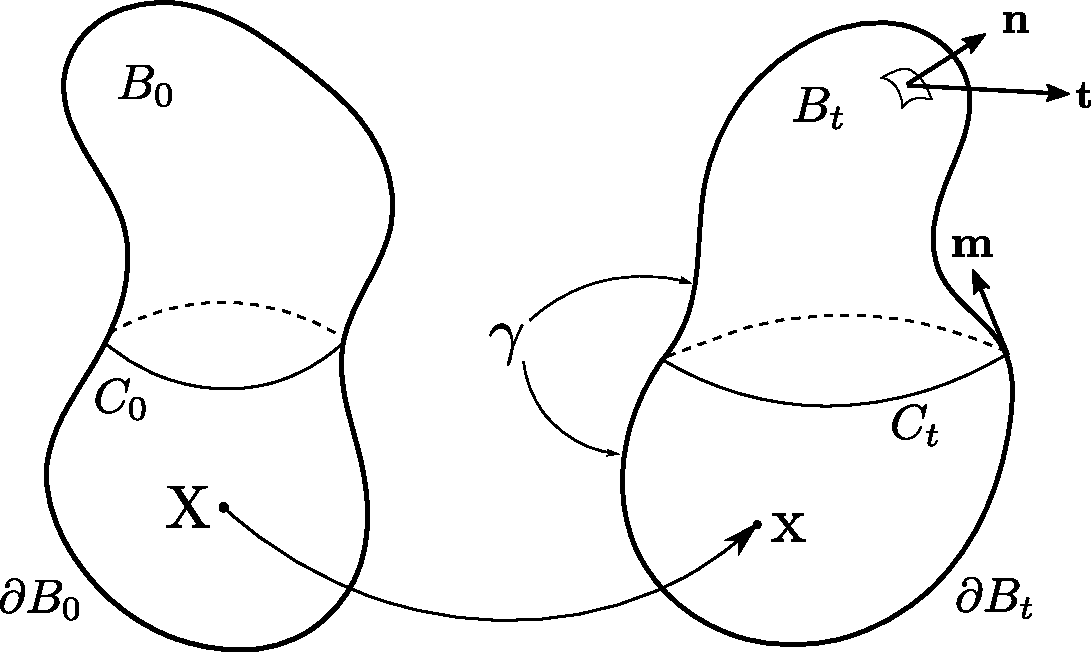
\includegraphics[scale=0.4]{pics/refdef.pdf}
\caption{The reference body $B_0$ and the deformed body $B_t$ at time $t$.}
\label{ref} \end{center}
\end{figure}

Using the~\citet{saksonoCM2006a} model, we begin with the force continuity at the solid-liquid interface, 
\begin{equation}\label{eq:sak1} {\sigma} \mbf{n}=-p_{ext}\mbf{n}+2H\gamma\mbf{n}
\end{equation}
where $\mbf{n}$ is the unit normal, $\sigma$ is the Cauchy stress, $H$ is the mean curvature, and $p_{ext}$ is an external pressure.  The spatial (updated Lagrangian) form of the weak form of the momentum equation can then be written as
\begin{dmath}\label{eq:sak2} \int (\sigma:\nabla\mbf{w}-\rho(\mbf{b-a})\cdot\mbf{w})dv-\int \mbf{t}\cdot\mbf{w}da-\int (-p_{ext}\mbf{n}\cdot\mbf{w})da \\ \nonumber
+\int (\gamma\nabla_{s}\cdot\mbf{w})da-\int (\gamma\mbf{w}\cdot\mbf{m})ds = 0
\end{dmath}
where $\mbf{w}$ is the virtual displacement, $\mbf{t}$ is the traction, $\mbf{b}$ is the body force, $\nabla_{s}=(\mbf{I}-\mbf{n}\otimes\mbf{n})\nabla$ is the surface gradient operator, $\rho$ is the density and $\mbf{a}$ is the acceleration.  In the present work, we neglect the three-phase contact line, i.e. the integral in (\ref{eq:sak2}) over the line $ds$, for simplicity.

The FE form of (\ref{eq:sak2}) can be obtained by making the usual Galerkin approximation of both the displacements and virtual displacements with the same shape functions, resulting in the (mechanical) residual $\mbf{R}^{mech}(\mbf{X})$
\begin{equation}\label{eq:sak3} \mbf{R}^{mech}(\mbf{X})=\mbf{M}\ddot{\mbf{X}}+\mbf{F}^{int}-\mbf{F}^{ext}+\mbf{F}^{surf}=0
\end{equation}
where the various terms in (\ref{eq:sak3}) take the following form for each element $e$
\begin{eqnarray}\label{eq:sak4} \mbf{M}_{e}=\int\rho\mbf{N}^{T}\mbf{N}dv \\ \nonumber
\mbf{F}_{e}^{int}=\int\mbf{B}^{T}\sigma dv \\ \nonumber
\mbf{F}_{e}^{ext}=\int\mbf{N}^{T}\mbf{b}dv + \int\mbf{N}^{T}\mbf{t}da \\ \nonumber
\mbf{F}_{e}^{surf}=\int\gamma\nabla_{s}\mbf{N}da
\end{eqnarray}
where $\mbf{N}$ and $\mbf{B}$ are the standard FE shape function and gradient, respectively.  As can be seen in (\ref{eq:sak3}), the only non-standard term compared to the standard discretization of the momentum equation arises in the surface force $\mbf{F}^{surf}$, and the corresponding surface stiffness $\mbf{K}^{surf}$.  

\begin{figure} \begin{center}
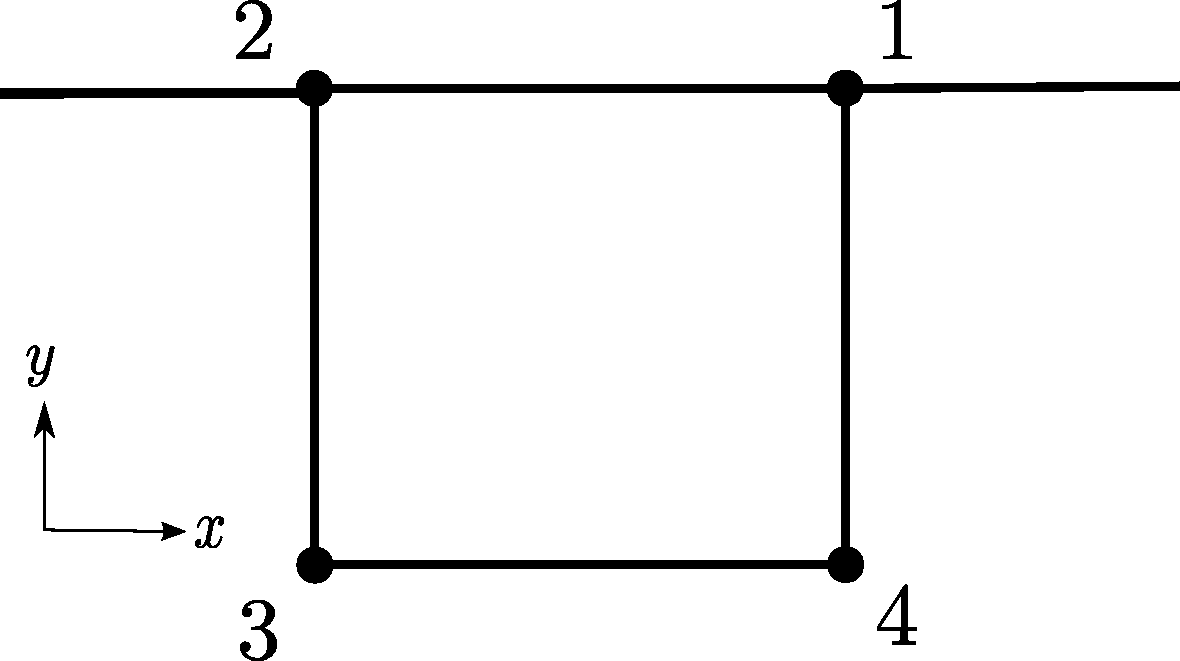
\includegraphics[scale=0.3]{pics/element.pdf}
\caption{Schematic of finite element nodal numbering consistent with surface tension formulation given in Eqs. (\ref{eq:sak5}) and (\ref{eq:sak6}).  Nodes 1 and 2 are surface nodes.}
\label{element} \end{center}
\end{figure}

~\citet{henannSM2014} analytically derived the surface force $\mbf{F}^{surf}$ for a two-dimensional, 4-node bilinear quadrilateral element as
\begin{equation}\label{eq:sak5} \mbf{F}^{surf}=-\frac{h\gamma}{L_{e}}\left(\begin{array}{cccc} {x_{1}-x_{2}} \\ {y_{1}-y_{2}} \\ {x_{2}-x_{1}} \\ {y_{2}-y_{1}} \end{array}\right)
\end{equation} 
The surface stiffness $\mbf{K}^{surf}$ can be obtained through linearization of the surface force $\mbf{F}^{surf}$ in (\ref{eq:sak3}).  This value for a 4-node bilinear quadrilateral element in two-dimensions was also given analytically by~\citet{henannSM2014} as
\begin{dmath} \label{eq:sak6} \mbf{K}^{surf}=\frac{h\gamma}{L_{e}}\left(\begin{array}{cccc} {1} & {0} & {-1} & {0} \\ {0} & {1} & {0} & {-1} \\ {-1} & {0} & {1} & {0} \\ {0} & {-1} & {0} & {1} \end{array}\right)-\frac{h\gamma}{L_{e}^{3}}\left(\begin{array}{cccc} {x_{1}-x_{2}} \\ {y_{1}-y_{2}} \\ {x_{2}-x_{1}} \\ {y_{2}-y_{1}} \end{array}\right)\left(\begin{array}{cccc} {x_{1}-x_{2}} \\ {y_{1}-y_{2}} \\ {x_{2}-x_{1}} \\ {y_{2}-y_{1}} \end{array}\right)^{T}
\end{dmath}
where $L_{e}$ is the length of the FE face containing nodes 1 and 2.  The ordering of the FE nodes corresponding to Eqs. (\ref{eq:sak5}) and (\ref{eq:sak6}) is shown in Figure (\ref{element}).  

The final coupled electromechanical FE equations we solve, which include the surface tension terms, can be written as
\begin{equation}\label{eq:sak7}\footnotesize{ \left(\begin{array}{cc}{\Delta\mbf{a}} \\ {\Delta\Phi}\end{array}\right)=-\left(\begin{array}{cc} {\mbf{M}+\beta\Delta t^{2}(\mbf{K}^{mm}+\mbf{K}^{surf})} & {\mbf{K}^{me}} \\ {\beta\Delta t^{2}\mbf{K}^{em}} & {\mbf{K}^{ee}} \end{array}\right)^{-1}\left(\begin{array}{cc}{\mbf{R}^{mech}} \\ {\mbf{R}^{elec}}\end{array}\right)}
\end{equation}
In comparing the new FE formulation including surface tension in (\ref{eq:sak7}) to the previous FE equations of~\citet{parkIJSS2012} in (\ref{eq:fe1}), the only changes are the addition of the surface stiffness $\mbf{K}^{surf}$ to the standard mechanical stiffness matrix $\mbf{K}^{mm}$, as well as the surface contribution $\mbf{F}^{surf}$ to the mechanical residual $\mbf{R}^{mech}$, as shown previously in (\ref{eq:sak3}) and (\ref{eq:sak4}).


\section{Numerical Results}


All numerical simulations were performed using the open source simulation code~\citet{tahoe} using standard 4-node, bilinear quadrilateral finite elements within a two-dimensional, plane strain approximation.  Before any application of electrostatic loading via applied voltages, the surface tension is first applied incrementally until the desired value is reached.  This incremental approach is necessary to avoid computational instabilities, as previously discussed by~\citet{javiliCMAME2010}.  The surface tension is applied incrementally by first defining a target value of surface tension $\gamma$, after which we are able to define the following function for the current value of surface tension $\gamma_{0}$: 
\begin{equation} \gamma_{0}=min\left(\gamma,\frac{\gamma t}{t_0}\right)
\label{eq:gammaramp}
\end{equation}
where $t$ is the current time and $t_0$ is the total time allotted to reach the prescribed value for surface tension $\gamma$.  Once the system is in equilibrium with the surface tension, voltage is applied in a monotonically increasing fashion.

\subsection{Single Element Tests}

We first perform a suite of parametric benchmark studies to gain a qualitative understanding of how surface tension impacts the electromechanical behavior of DEs undergoing homogeneous and inhomogeneous deformation.  A single 4-node bilinear quadrilateral element of unit length and height is used for these simulations.  For all numerical simulations, we chose the following constitutive parameters for the Arruda-Boyce model in Eq. (\ref{eq:de2}):  $\mu=\epsilon=1$, $\lambda=1000$ and $N=5.0$, while different values of the surface tension $\gamma$ are chosen. 

\subsubsection{Homogeneous Deformation}

\begin{figure} \begin{center} 
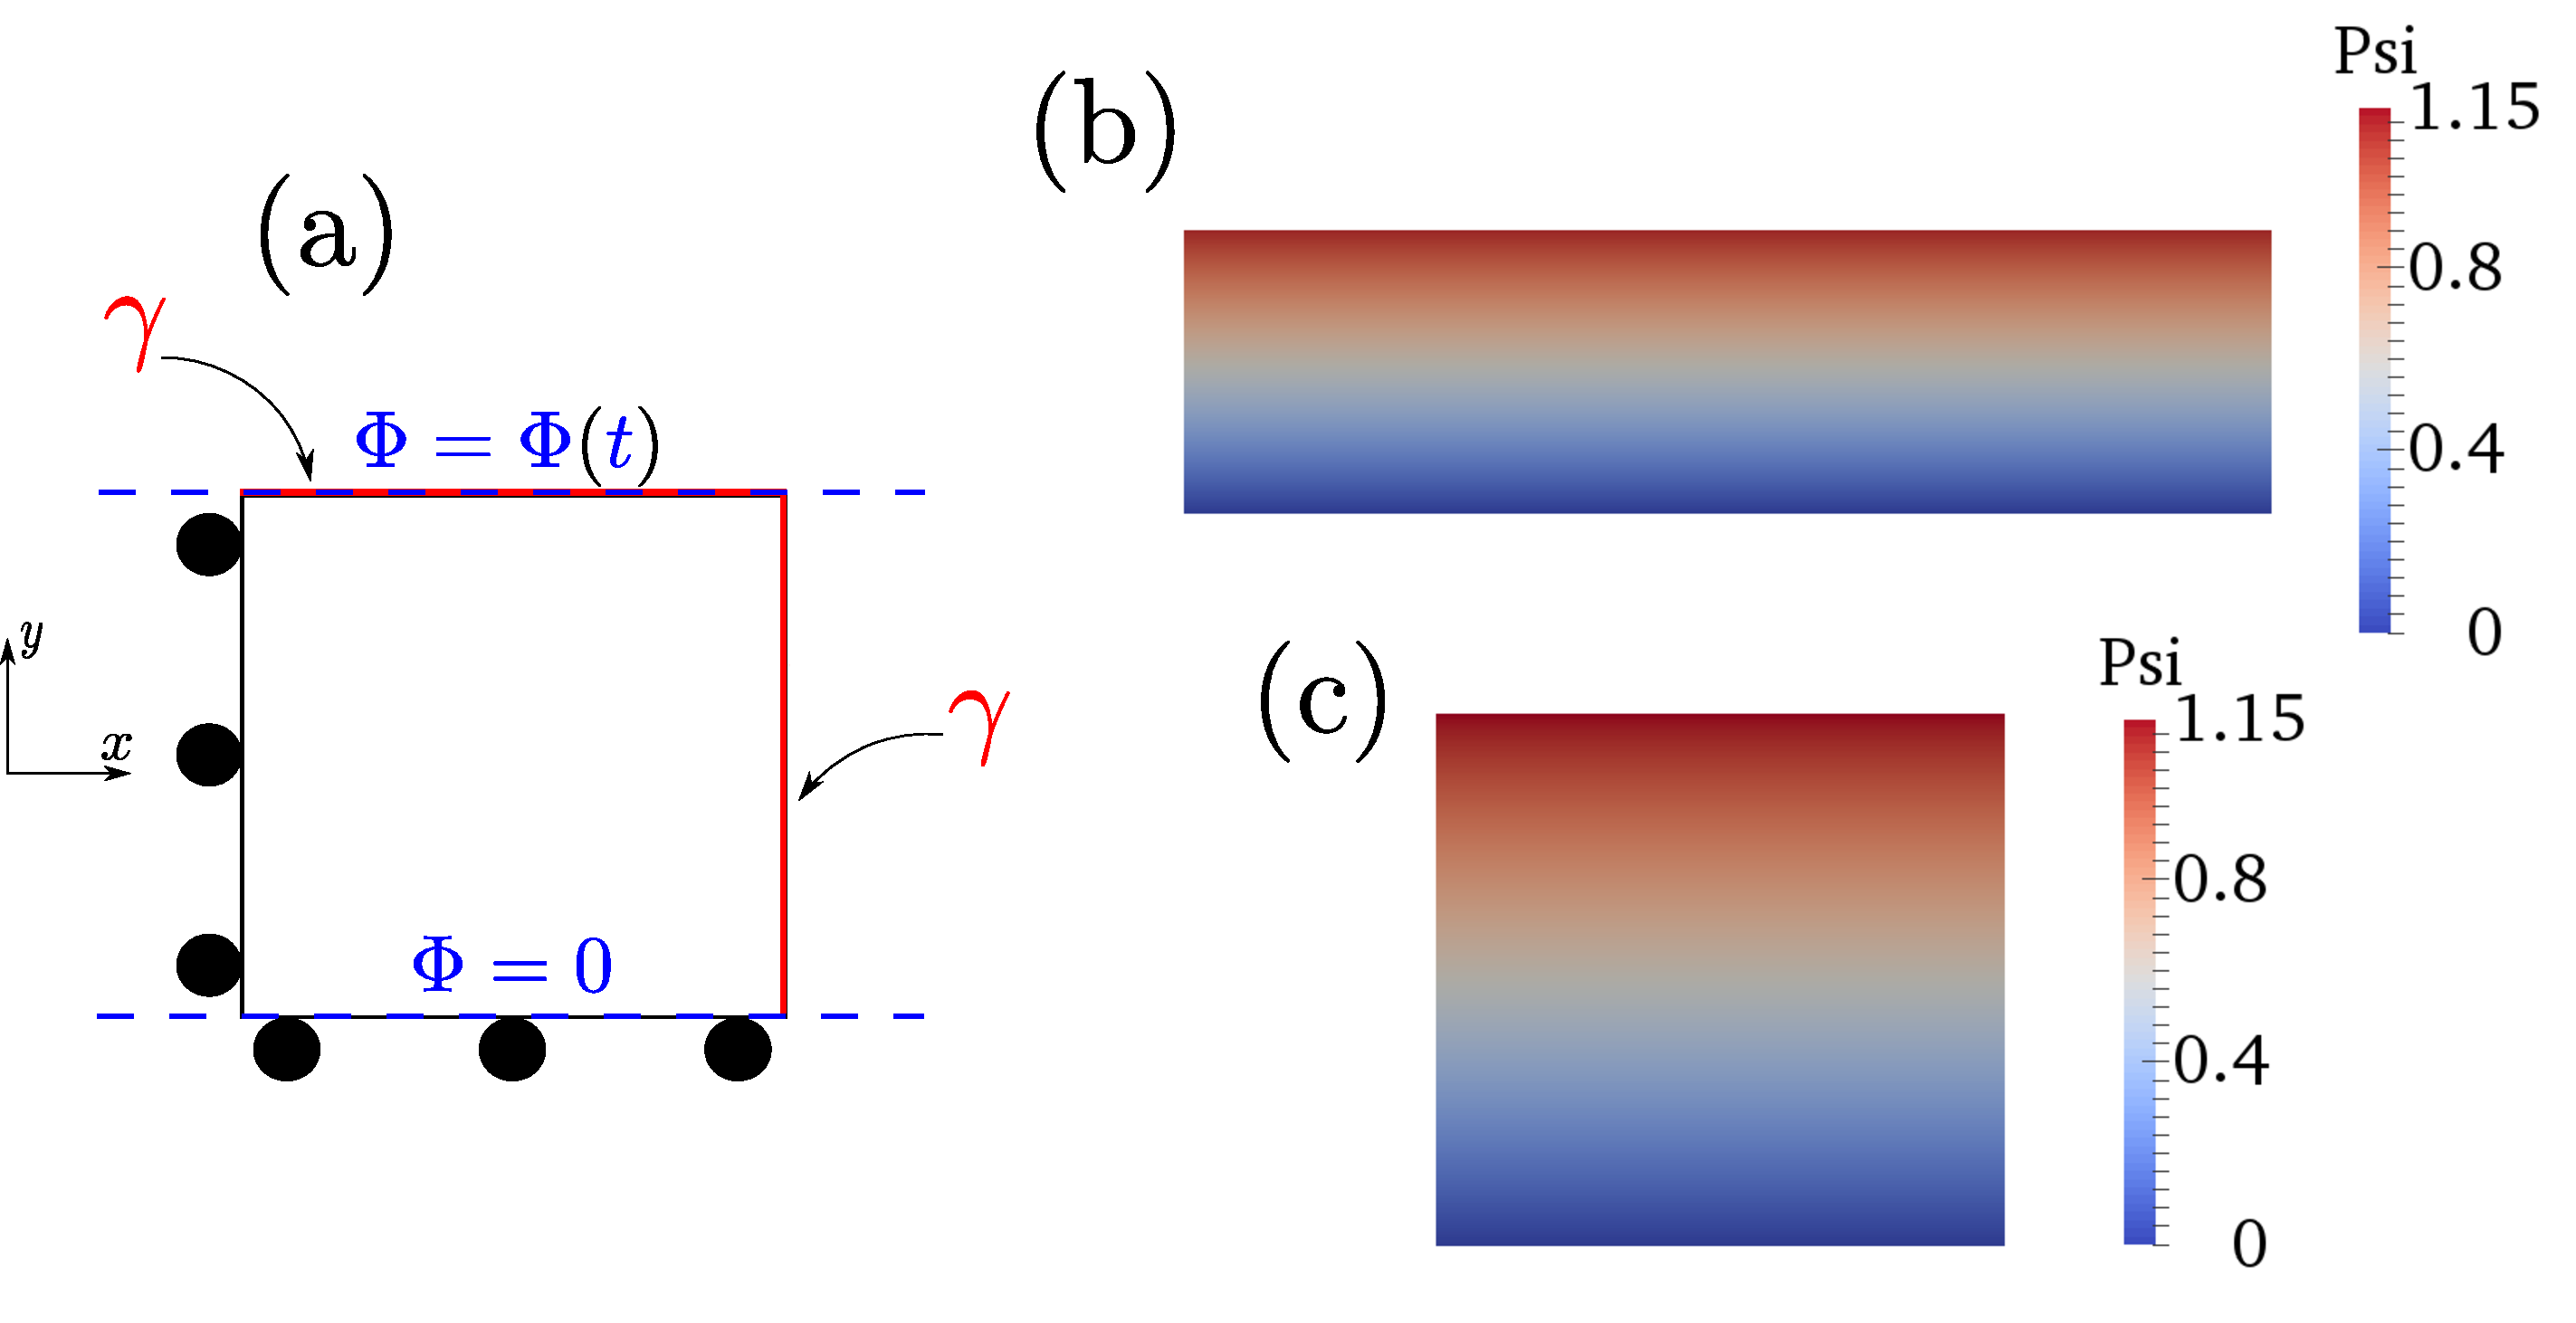
\includegraphics[scale=0.25]{pics/homo3.pdf}
\caption{(a) Schematic of a single finite element with homogeneous boundary conditions; (b) Deformed configuration with $\gamma/\mu l=0$; (c) Deformed configuration with $\gamma/\mu l=10$.  \hsp{Note that Psi in (b) and (c) refers to voltage.}}
\label{homo3} \end{center} \end{figure}

The first set of boundary conditions are to allow homogeneous deformation of the DE. The electromechanical boundary conditions are as shown in Fig. (\ref{homo3})(a), with rollers on the -x and -y surfaces, and voltage applied at the top surface of the single square element.  \hsp{Surface tension is present on the free surfaces.}  The resulting configurations for elastocapillary number values of $\gamma/\mu l=0$ and $\gamma/\mu l=10$ are shown in Figures (\ref{homo3})(b) and (c).  As can be seen, Figure (\ref{homo3})(b) shows the well-known deformed configuration where the DE contracts along the thickness direction while simultaneously elongating in response to the applied voltage, thus exhibiting the well-known electromechanical snap through instability~\cite{parkIJSS2012}.  However, the configuration in Figure (\ref{homo3})(c) is quite different when $\gamma/\mu l=10$.  Instead of resulting in a rectangular deformed configuration, the single element takes a deformed configuration that is not much changed from the initial, square configuration, which shows that the impact of surface tension is to resist the deformation that would otherwise occur due to the applied voltage.

We plot the resulting normalized voltage-charge curves in Figure (\ref{homo}) for various values of $\gamma/\mu l$.  We can see that the effect of increasing surface tension is to significantly increase the voltage that is required to induce the electromechanical instability.  These results are quantitatively in agreement with previous experimental and theoretical studies on soft materials which found that the effect of surface tension is to create a barrier to instability nucleation~\citep{chenPRL2012,moraSM2011}.  We also note that a softening response is not observed in the voltage-charge plot due the fact that a plane strain, and not plane stress~\citep{zhouIJSS2008} approximation in two dimensions is utilized. 

%\begin{figure} \begin{center} 
%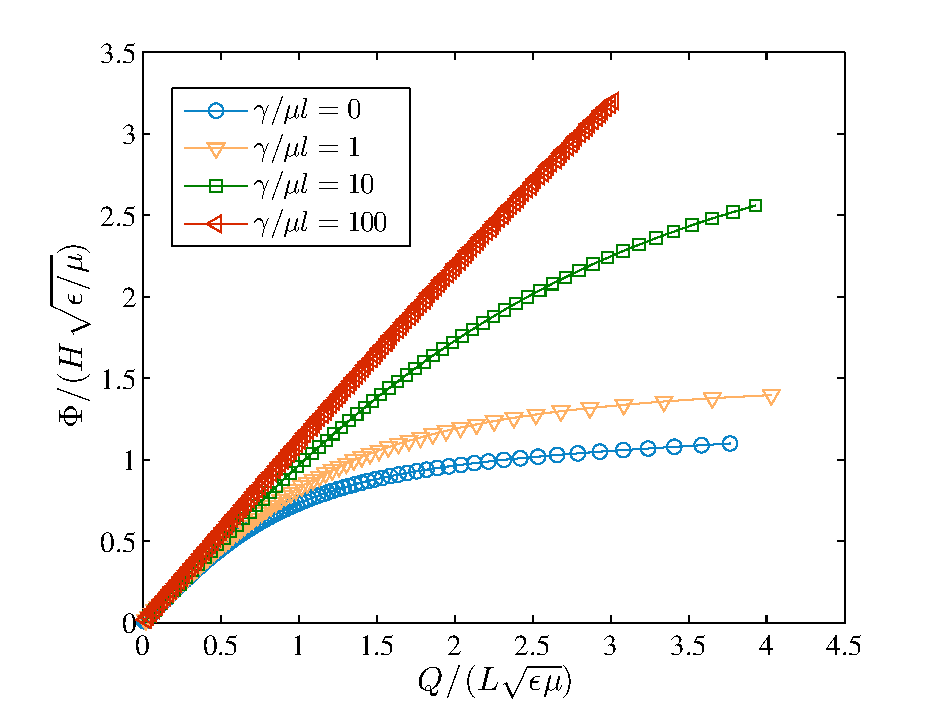
\includegraphics[scale=0.6]{pics/voltage_hom.pdf}
%\caption{Deformation of a single, homogeneously deforming finite element subject to voltage loading.}  
%\label{homo} \end{center} \end{figure}
\begin{figure}
\centering
\begin{tikzpicture}
	\begin{axis}[
		xmin=0,
		ymin=0,
		xlabel=$Q/(L\sqrt{\epsilon\mu})$,
		ylabel=$\Phi/(H\sqrt{\epsilon/\mu})$,
		legend pos=north west,
		legend entries={$\gamma/\mu l=0$,$\gamma/\mu l=1$,$\gamma/\mu l=10$,$\gamma/\mu l=100$}]
	\addplot+[mark repeat=3] table {data/homogen/v1.dat};
	\addplot+[mark repeat=3] table {data/homogen/v2.dat};
	\addplot+[mark repeat=3] table {data/homogen/v3.dat};	
	\addplot+[mark repeat=3] table {data/homogen/v4.dat};
	\end{axis} 
\end{tikzpicture}
	\caption{Deformation of a single, homogeneously deforming finite element subject to voltage loading.}
	\label{homo}
\end{figure}



\subsubsection{Inhomogeneous Deformation}

\begin{figure} \begin{center} 
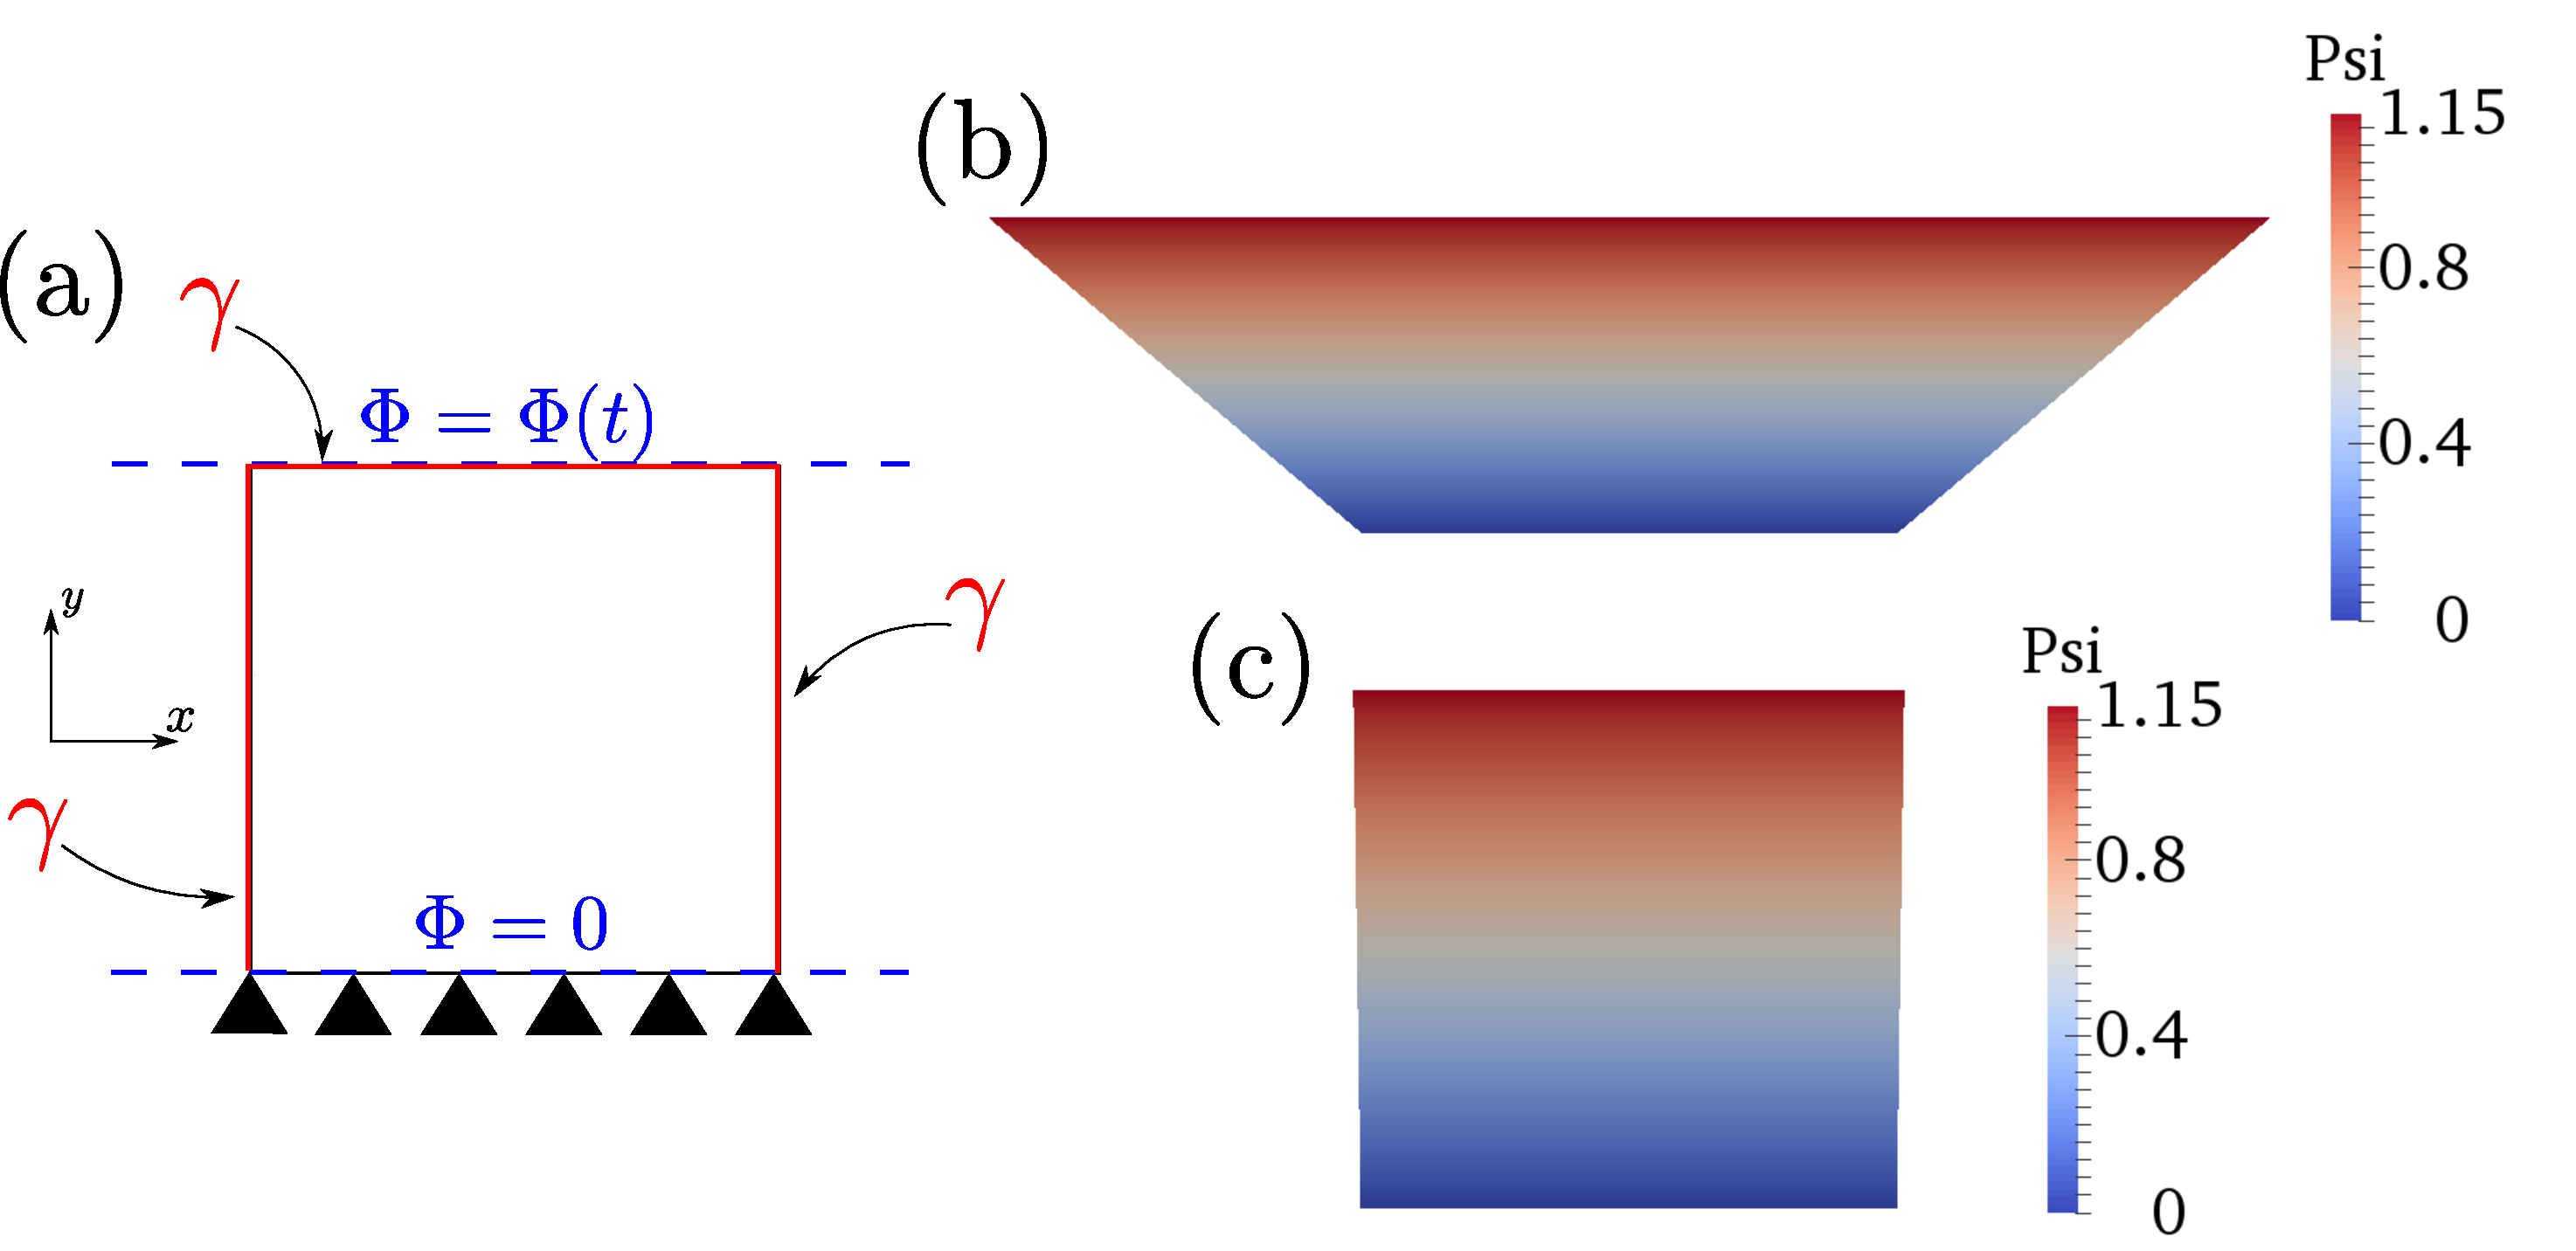
\includegraphics[scale=0.25]{pics/inhomo3.pdf}
\caption{(a) Schematic of single finite element with inhomogeneous boundary conditions; (b) Deformed configuration with $\gamma/\mu l=0$; (c) Deformed configuration with $\gamma/\mu l=10$.  \hsp{Note that Psi in (b) and (c) refers to voltage.}}  
\label{inhomo3} \end{center} \end{figure}


Before studying surface tension effects on inhomogeneously deforming DEs, as will be done in subsequent computational examples, we first study a single FE that is fully constrained mechanically along its bottom surface, as illustrated in Figure (\ref{inhomo3})(a), \hsp{where surface tension is present on the free surfaces}.  If no surface tension is present, i.e. $\gamma/\mu l=0$, the top surface of the element bows outward in response to the applied voltage as seen in Figure (\ref{inhomo3})(b).  However, for non-zero surface tension $\gamma/\mu l=10$, the large outward bowing of the top surface that was observed for $\gamma/\mu l=0$ in Figure (\ref{inhomo3})(b) is reduced drastically, as shown in Figure (\ref{inhomo3})(c).  The effect of the surface tension opposing the deformation that is induced by the voltage is similar to that previously observed for the homogeneous boundary conditions.

%\begin{figure} \centering 
%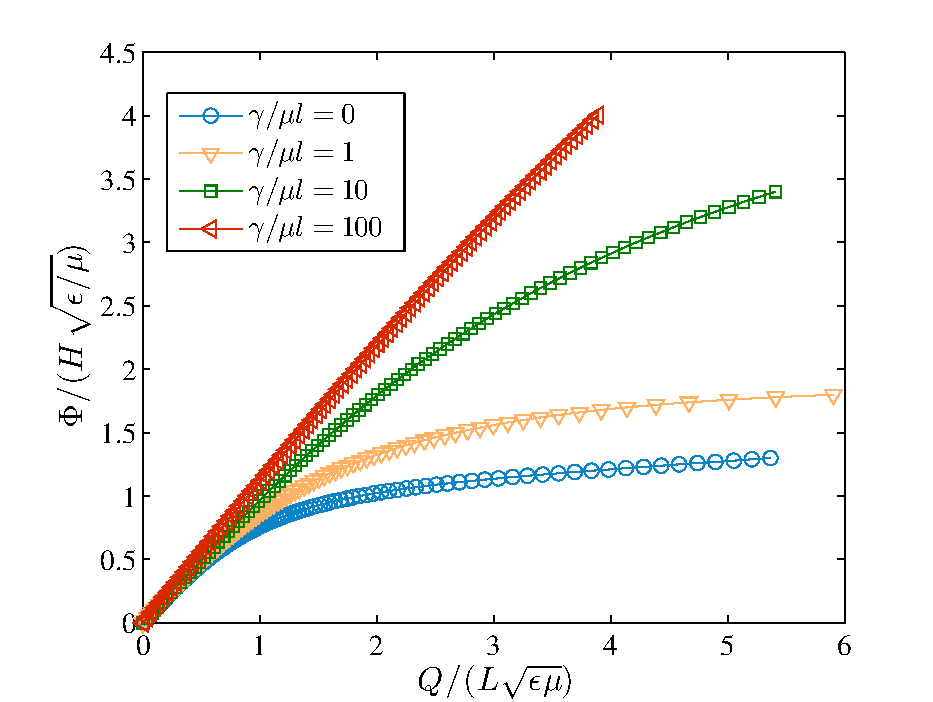
\includegraphics[scale=0.6]{pics/voltage_inhom.pdf}
%\caption{Deformation of a single, inhomogeneously deforming finite element subject to voltage loading.}    
%\label{inhomo}  \end{figure}

\begin{figure}
\centering
\begin{tikzpicture}
	\begin{axis}[
		xmin=0,
		ymin=0,
		xlabel=$Q/(L\sqrt{\epsilon\mu})$,
		ylabel=$\Phi/(H\sqrt{\epsilon/\mu})$,
		legend pos=north west, 
		legend entries={$\gamma/\mu l=0$,$\gamma/\mu l=1$,$\gamma/\mu l=10$,$\gamma/\mu l=100$}]
	\addplot+[mark repeat=3] table {data/inhomogen/v1.dat};
	\addplot+[mark repeat=3] table {data/inhomogen/v2.dat};
	\addplot+[mark repeat=3] table {data/inhomogen/v3.dat};	
	\addplot+[mark repeat=3] table {data/inhomogen/v4.dat};
	\end{axis} 
\end{tikzpicture}
	\caption{Deformation of a single, inhomogeneously deforming finite element subject to voltage loading.}
	\label{inhomo}
\end{figure}

We also analyze the voltage-charge curve for different values of $\gamma/\mu l$ in Figure (\ref{inhomo}).  As can be seen, the major effect of surface tension is again to significantly increase the value of voltage $\Phi$ that is required in order to induce the voltage-induced electromechanical snap-through instability.

\subsection{Surface Creasing in Constrained 2D Strip}

Our next example is based on recent experiments by~\citet{wangPRE2013}, who studied the surface instability mechanisms in constrained DE films in which the top surface is immersed in a fluid.  The fluid was varied such that the top surface of the DE film was subject to different values of surface tension.  Interestingly, upon application of a critical voltage, a transition in the surface instability mechanism from creasing to wrinkling was observed, which was found to be dependent on elastocapillary length $\gamma/(\mu H)$.  Along with the transition in surface instability mechanism, the wavelength of the instability was also found to change, from about $\lambda=1.5H$ for the creasing instability to longer wavelengths, $\lambda=5-12H$ when the elastocapillary length $\gamma/(\mu H)>1$.  

We performed FE simulations of the experiments of~\citet{wangPRE2013}, where the schematic of the problem geometry and the relevant electro-elasto-capillary boundary conditions is shown in Figure (\ref{film}), i.e. the bottom surface of the film is fixed, the left and right sides are on rollers while a voltage is applied to the top surface, where the surface tension is also present.   Most results shown are for a DE film of dimensions 160x4, which was discretized with square finite elements having an edge length of unity.

\begin{figure} \begin{center} 
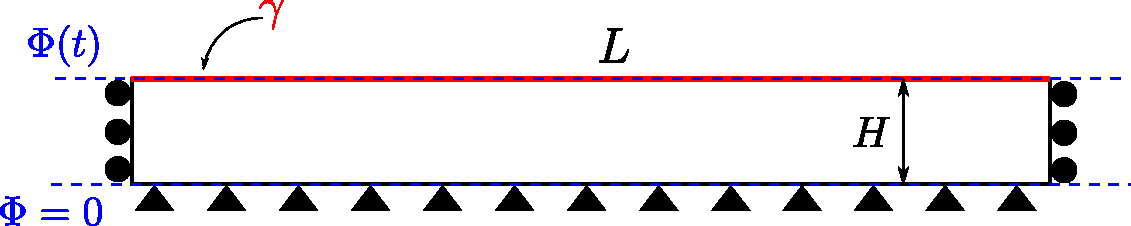
\includegraphics[scale=0.6]{pics/film.pdf}
\caption{Schematic of the DE film with electro-elasto-capillary boundary conditions.}
\label{film} \end{center} \end{figure}

\begin{figure} \begin{center} 
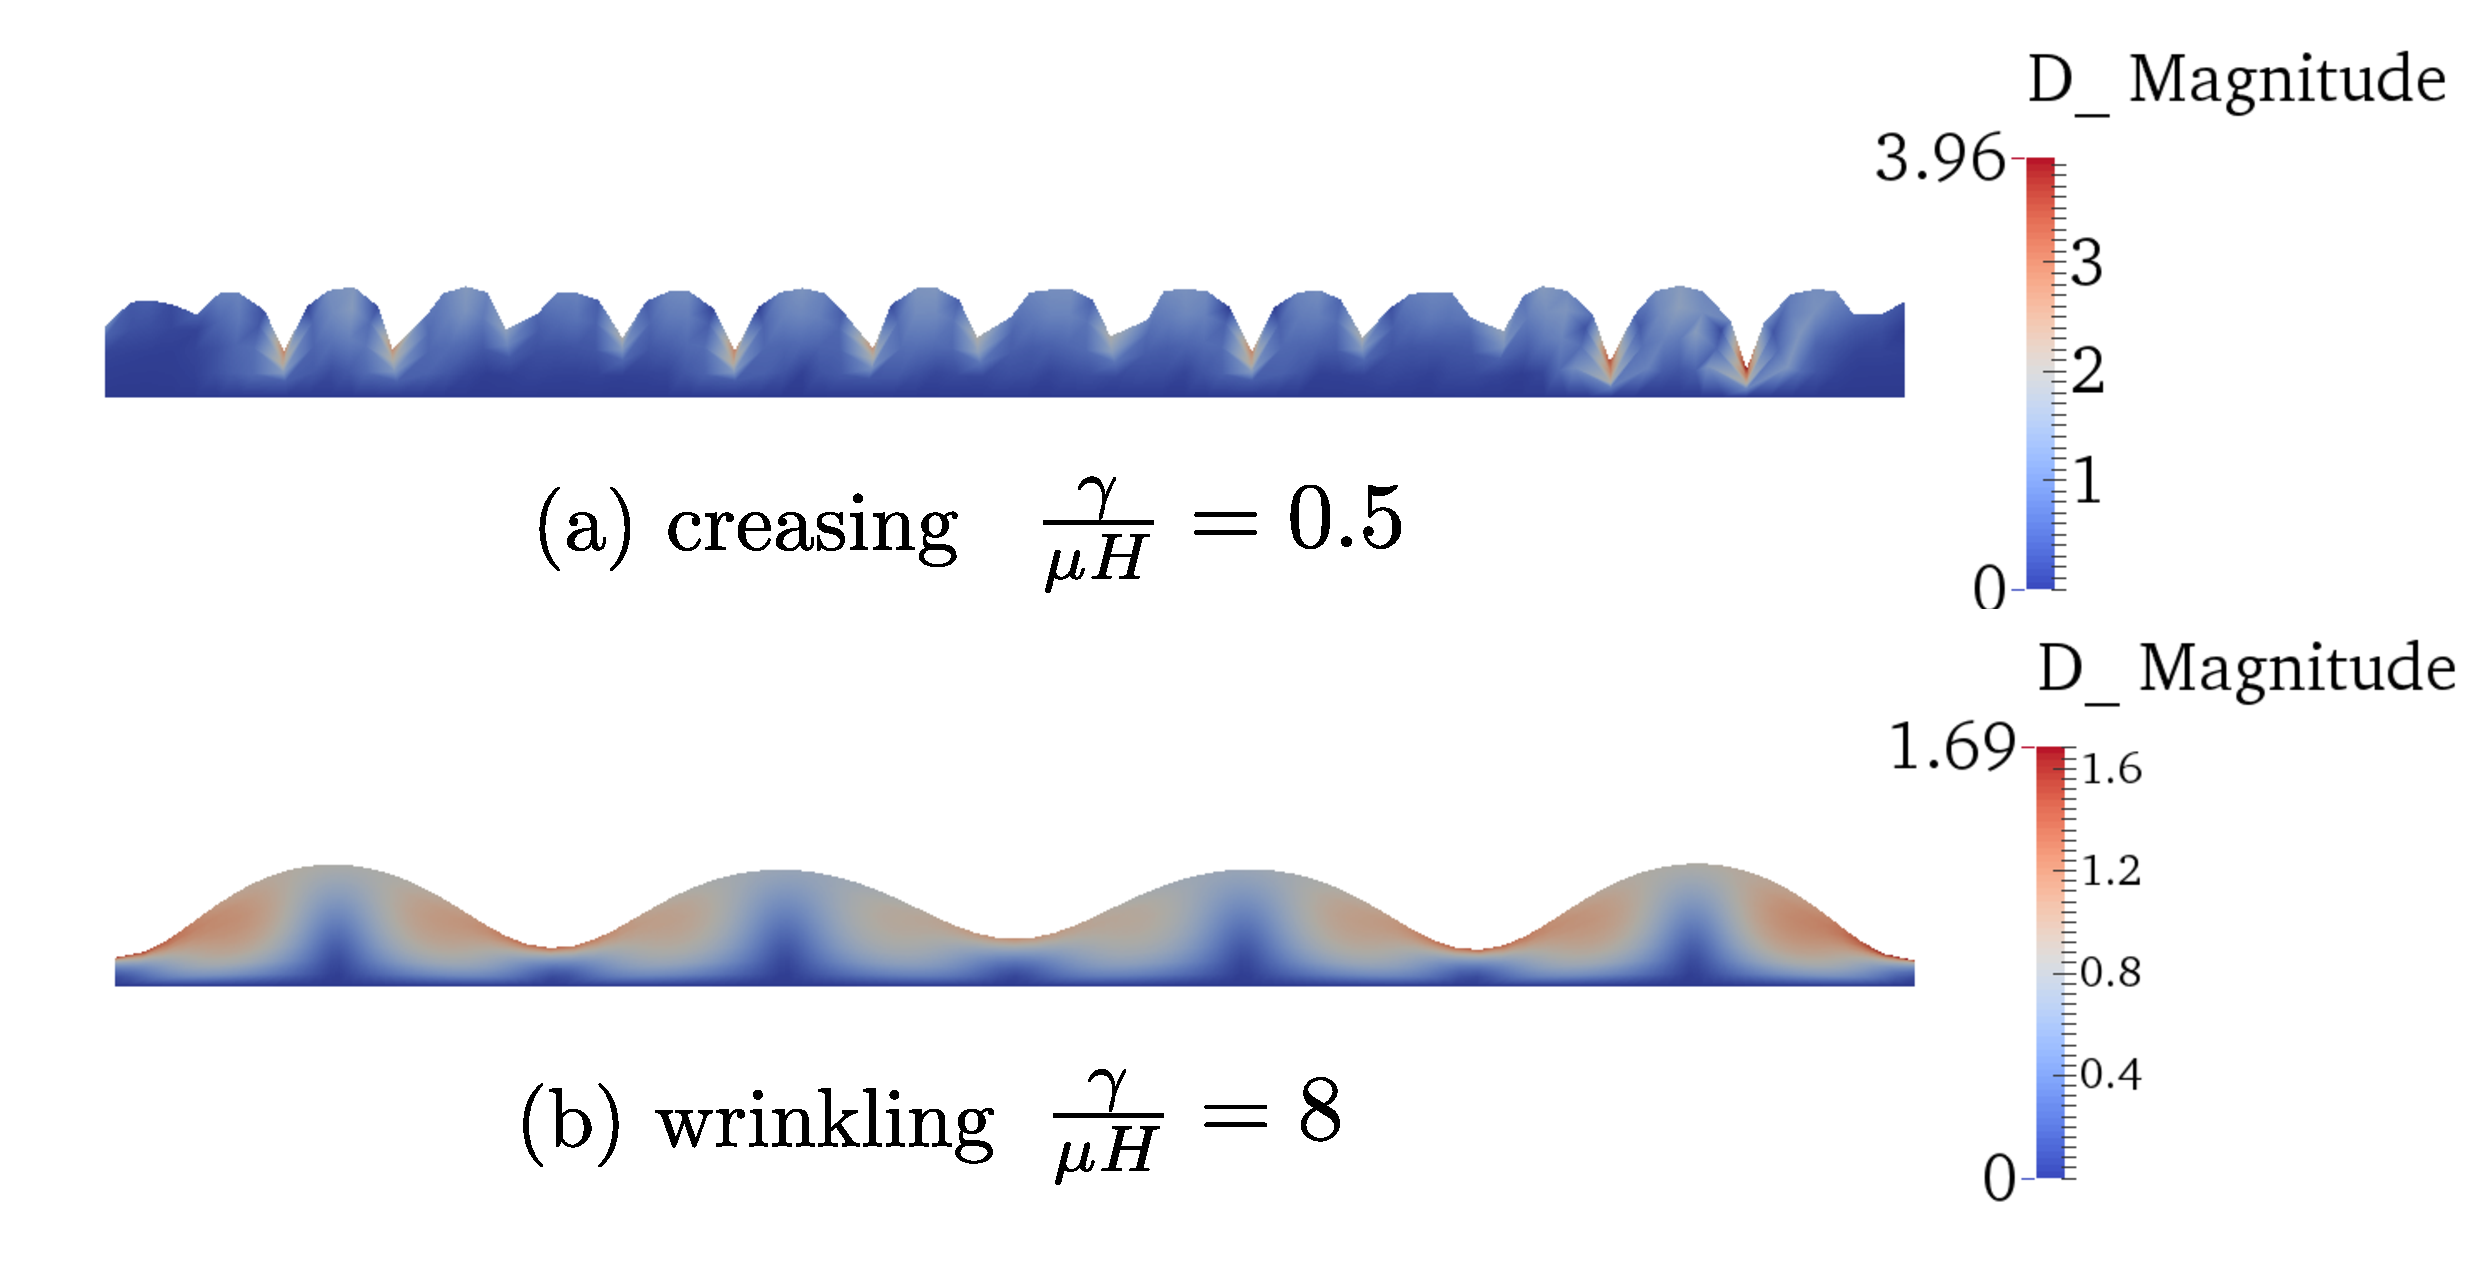
\includegraphics[scale=0.35]{pics/wrinkcreas.pdf}
\caption{Computationally observed transition in the surface instability mechanism in DEs as a function of the elastocapillary length $\gamma/(\mu H)$, for a DE film of dimensions 80x4.  \hsp{The variable D_Magnitude refers to the magnitude of the displacement field.}}
\label{wrinkcreas} \end{center} \end{figure}

We show in Figure (\ref{wrinkcreas})(a) the difference in surface instability mechanism depending on the elastocapillary length.  As can be seen, when the elastocapillary length is small (i.e. $\gamma/\mu H=0.5$), the surface instability mechanism is that of creasing, or localized folds.  As the elastocapillary length increases to become similar to the film height, the surface instability mechanism changes to wrinkling, as shown in Figure (\ref{wrinkcreas})(b).  The change in instability mechanism is characterized by a significantly larger instability wavelength as compared to the creasing instability in Figure (\ref{wrinkcreas})(a).  Furthermore, rather than abrupt, localized folds as in the creasing instability in Figure (\ref{wrinkcreas})(a), the surface exhibits a more gradual and undulating pattern as seen in Figure (\ref{wrinkcreas})(b).  

%\begin{figure} \centering 
%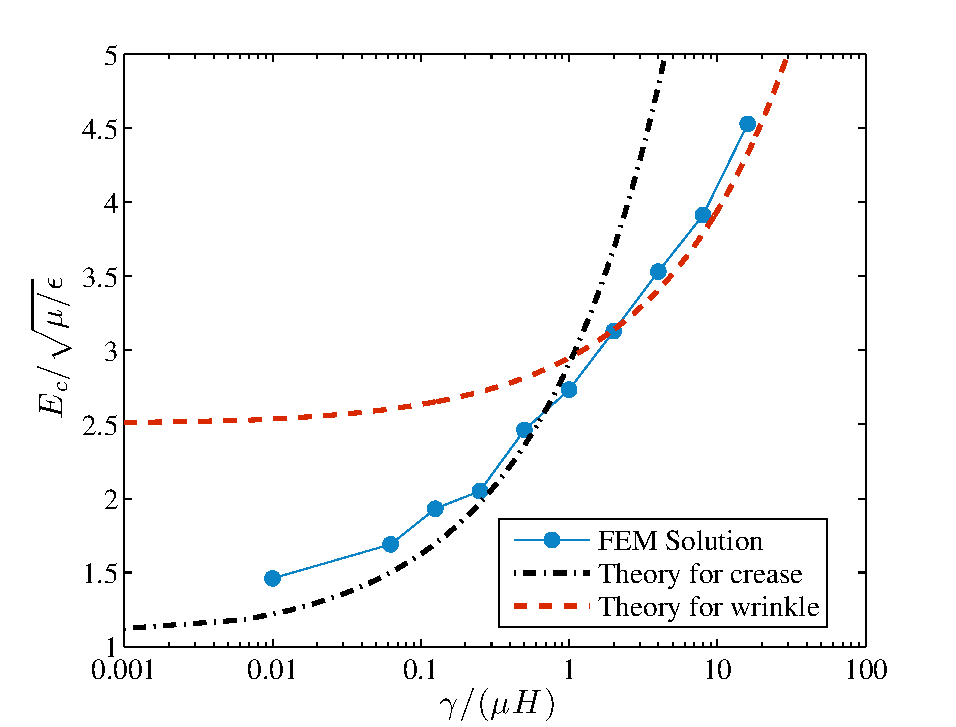
\includegraphics[scale=0.58]{pics/Ec.pdf}
%\caption{Normalized critical electrical field as a function of elastocapillary length for a 160x4 DE film.}   
%\label{ecrit2} \end{figure}

\begin{figure}
\centering
\begin{tikzpicture}
	\begin{axis}[
		xmode=log,
		xmin=0.001,
		ymax=5,
		xlabel=$\gamma/(\mu H)$,
		ylabel=$E_{c}\sqrt{\mu/\epsilon}$,
		legend pos=north west, 
		legend entries={FEM Solution,Theory for crease,Theory for wrinkle}]
	\addplot+[mark repeat=1] table {data/Ec/Ec1.dat};	
	\addplot+[mark=none, dash pattern=on 4pt off 1pt on 4pt off 4pt] table {data/Ec/Ec2.dat};	
	\addplot+[mark=none, dash pattern=on 2pt off 1pt on 2pt off 2pt] table {data/Ec/Ec3.dat};	
	\end{axis} 
\end{tikzpicture}
	\caption{Normalized critical electrical field as a function of elastocapillary length for a 160x4 DE film.}
	\label{ecrit2}
\end{figure}

This instability transition was also characterized experimentally by plotting the normalized electric field $E_{c}/\sqrt{\mu/\epsilon}$  as a function of the elastocapillary length~\cite{wangPRE2013}, as shown in Figure (\ref{ecrit2}), where $E_{c}$ is the value of the electric field when the instability nucleates.  The analytic solutions for the critical electric fields to nucleate wrinkles and creases were developed by~\citet{wangPRE2013}, and can be written as:  
\begin{equation} \label{eqn:ECcrease}
E^{c}_{crease}\approx1.03\sqrt{\frac{\mu}{\epsilon}}+1.88\sqrt{\frac{\gamma}{H\epsilon}}
\end{equation}
\begin{equation} \label{eqn:ECwrinkle}
E^{c}_{wrinkle}\approx2.49\sqrt{\frac{\mu}{\epsilon}}+0.46\sqrt{\frac{\gamma}{H\epsilon}}
\end{equation}
As seen in Figure (\ref{ecrit2}), the FE model is able to capture the general trends, including the transition in the value of the critical electric field $E_{c}$ predicted theoretically.  The FE prediction for the critical electric field is generally larger than the analytic theory, which is expected given that while a locking-resistant Q1P0 formulation was used~\cite{simoCMAME1985}, the FE-discretized structure is still stiffer than the continuum.  

%\begin{figure} \centering 
%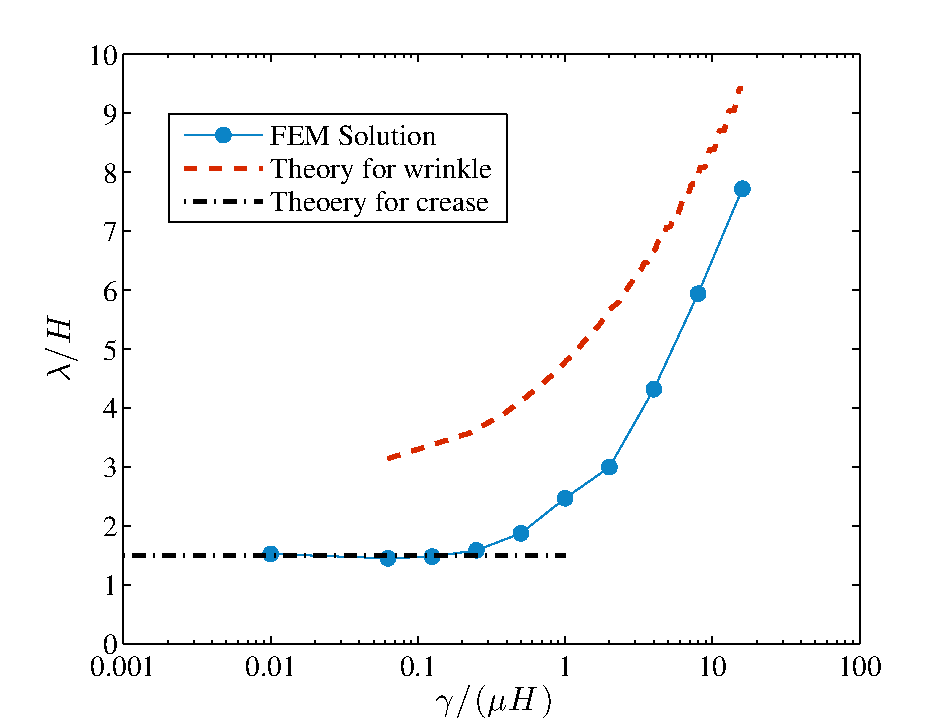
\includegraphics[scale=0.58]{pics/wave.pdf}
%\caption{Normalized instability wavelength as a function of elastocapillary length for a 160x4 DE film.}
%\label{ecrit1} \end{figure}

\begin{figure}
\centering
\begin{tikzpicture}
	\begin{axis}[
		xmode=log,
		xmin=0.001,
		ymax=10,
		xlabel=$\gamma/(\mu H)$,
		ylabel=$\lambda/(H)$,
		legend pos=north west, 
		legend entries={FEM Solution,Theory for crease,Theory for wrinkle}]
	\addplot+[mark repeat=1] table {data/wave/W1.dat};	
	\addplot+[mark=none, dash pattern=on 4pt off 1pt on 4pt off 4pt] table {data/wave/W2.dat};	
	\addplot+[mark=none, dash pattern=on 2pt off 1pt on 2pt off 2pt] table {data/wave/W3.dat};	
	\end{axis} 
\end{tikzpicture}
	\caption{Normalized instability wavelength as a function of elastocapillary length for a 160x4 DE film.}
	\label{ecrit1}
\end{figure}

We also calculated the normalized instability wavelength $\lambda/H$ as a function of the elastocapillary length as shown in Figure (\ref{ecrit1}).  In that figure, the wrinkling wavelength as a function of elastocapillary number is given by
\begin{equation} \label{eqn:wrinkle}
\frac{\epsilon E^2}{\mu}=2Hk\frac{1+2e^{2Hk}+e^{4Hk}+4e^{2Hk}H^2k^2}{-1+e^{4hk}-4e^{2Hk}Hk}+\left(Hk\right)^2\frac{\gamma}{\mu H}
\end{equation}
The creasing wavelength is fixed as $\lambda_{crease}=1.5H$, which was previously obtained by~\citet{wangPRE2013}.

For elastocapillary numbers $\gamma/(\mu H)<1$, we find the normalized wavelength $\lambda/H$ to be close to the value of 1.5 predicted theoretically~\cite{wangPRE2013}.  For larger elastocapillary numbers, i.e. $\gamma/(\mu H)>1$, where wrinkling is observed, a dramatic increase in normalized instability wavelength $\lambda/H$ is observed.  While our FE simulations capture the instability wavelength transition, the predicted wavelength after the transition to wrinkling occurs is smaller than the analytic theory.  

This discrepancy was also observed in the experimental studies of~\citet{wangPRE2013}.  In that work, like the current FE models, the critical electric fields for creasing and wrinkling as in Figure (\ref{ecrit2}) were in better agreement with the analytic theory than the instability wavelength.  Specifically, the experiments also found a smaller instability wavelength in the transition region from creasing to wrinkling than the analytic solution.  The FE predictions do fall within the bounds observed experimentally by~\citet{wangPRE2013}, though at the lower end of the observed wavelengths.  This is likely due to differences in how the instability wavelength was calculated in our plane strain 2D FE simulations as compared to the 3D experimental studies.  In particular, there is larger spatial variation in the wavelengths observed in the 3D experimental structure, whereas the 2D plane strain approximation results in a constant instability wavelength through the thickness of the film, and so we expect and find that the FE predictions fall towards the lower end of the experimental values.

\subsection{Bursting drops in a dielectic elastomer}

\begin{figure} \begin{center} 
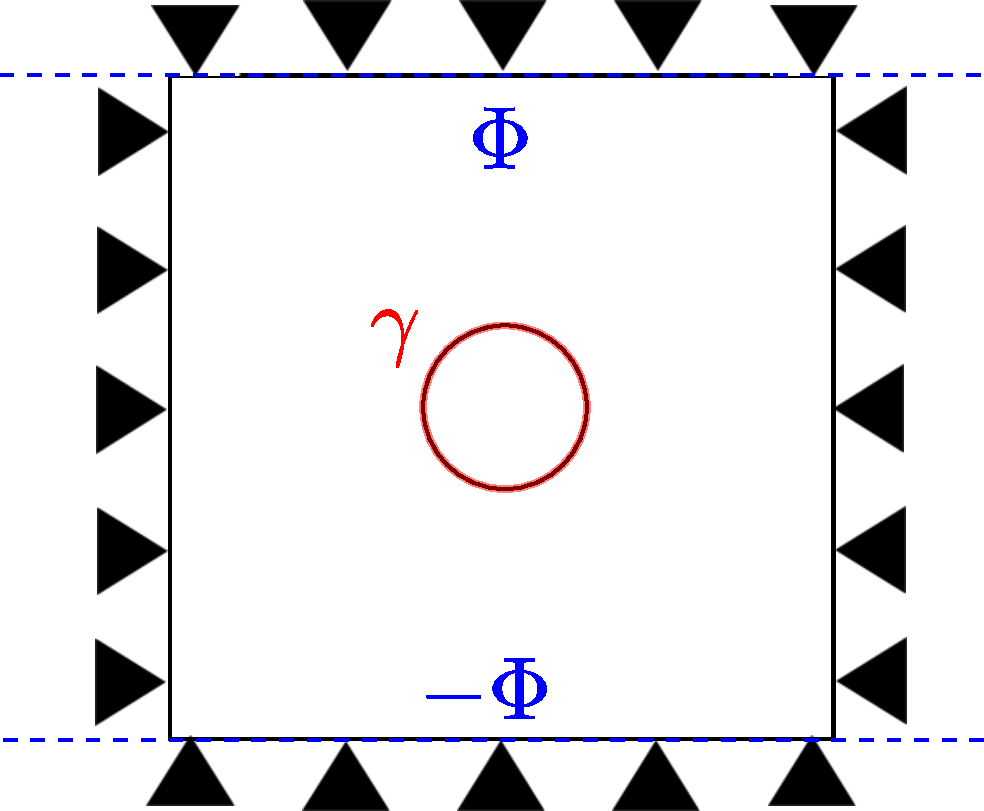
\includegraphics[scale=0.35]{pics/bursting2.pdf}
\caption{Computational model for bursting drop in dielectric elastomer} 
\label{burstingschematic} \end{center} \end{figure}

\begin{figure}
\centering
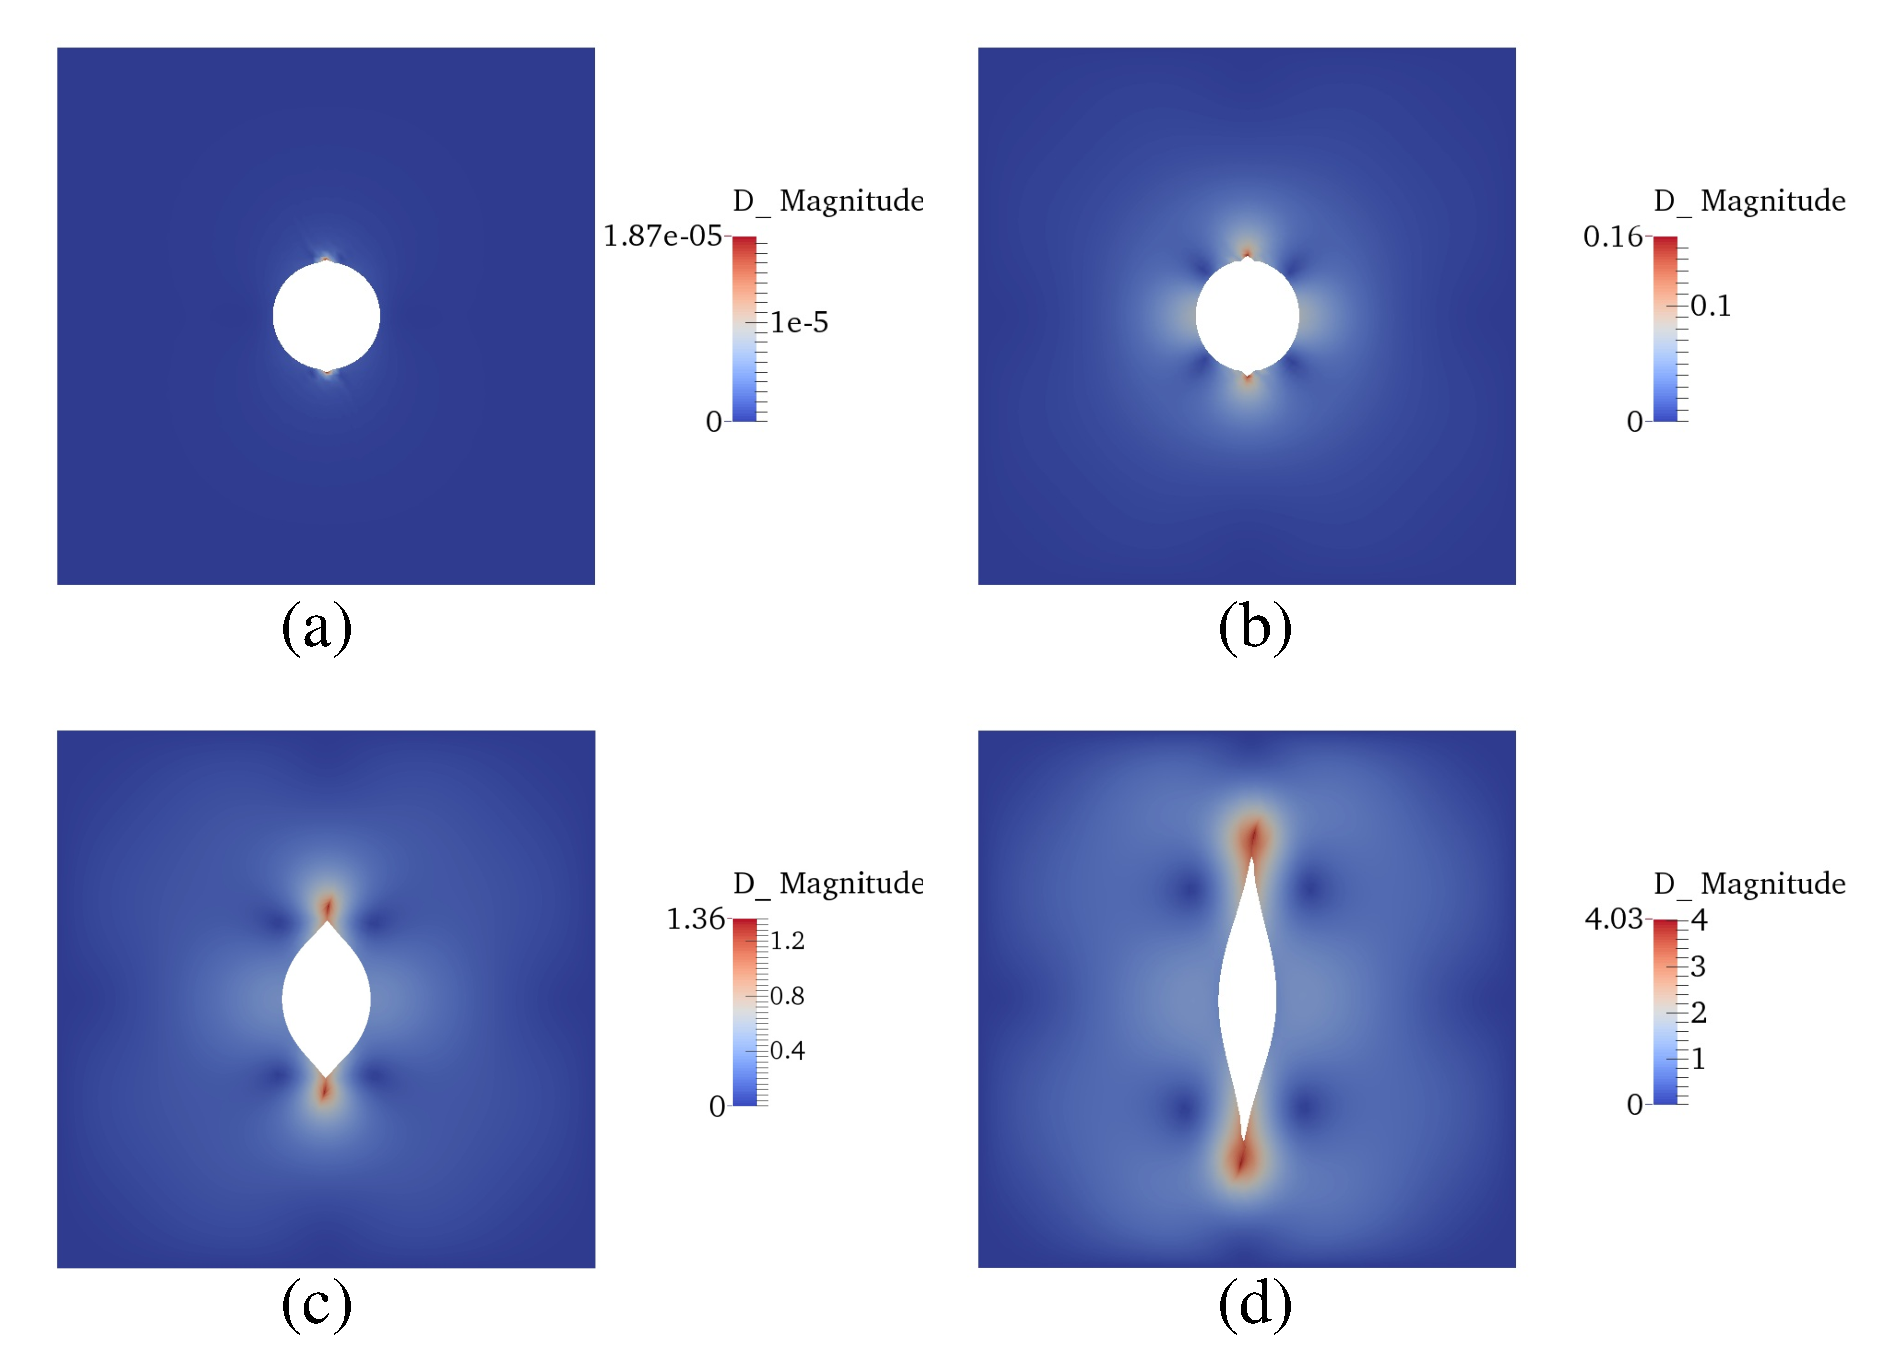
\includegraphics[scale=0.48]{pics/bursting1.eps}
\caption{Representative snapshots of crack propagation in constrained DE film}
\label{bursting1} \end{figure}

\begin{figure}
\begin{center}
\begin{tikzpicture}
	\begin{axis}[
		xmin=0,
		ymin=0,
		xlabel=$E_{top}\sqrt{\epsilon/\mu}$,
		ylabel=$b/R_0$,
		legend pos=north west,
		legend entries={$\gamma/\mu L=0$,$\gamma/\mu L=1$,$\gamma/\mu L=3$,$\gamma/\mu L=5$}]
	\addplot+[mark repeat=3] table {data/crack/gamma1.dat};
	\addplot+[mark repeat=3] table {data/crack/gamma2.dat};

	\addplot+[mark repeat=3] table {data/crack/gamma4.dat};
	
	\addplot+[mark repeat=3] table {data/crack/gamma6.dat};
	\end{axis}
\end{tikzpicture}
\end{center}
\caption{Deformation and instability of a single drop of conductive liquid in a dielectric elastomer under electric field}
\label{crack}
\end{figure}

\section{Conclusions}

We have presented a new dynamic, finite deformation finite element model of dielectric elastomers that incorporates surface tension to capture elastocapillary effects on the electromechanical deformation.  The simulations demonstrate that increasing surface tension, or equivalently the elastocapillary number, results in an increase in the critical voltage or electric field needed to nucleate an electromechanical instability in the dielectric elastomer.  We also demonstrated a transition in surface instability mechanism from creasing to wrinkling in constrained dielectric elastomer films by increasing the elastocapillary number.  The present results indicate that the proposed methodology may be beneficial in studying the electromechanical deformation and instabilities for dielectric elastomers in the presence of surface tension.

\section{Acknowledgements}

HSP and SS acknowledge funding from the ARO, grant W911NF-14-1-0022.

\section{Appendix}

%\begin{figure} \begin{center} 
%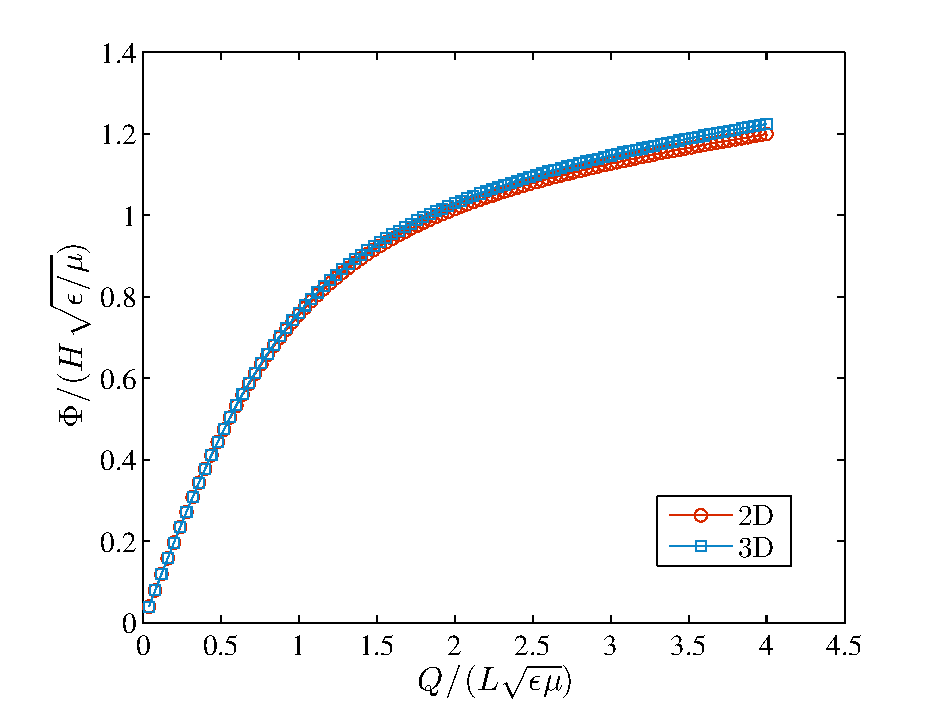
\includegraphics[scale=0.58]{pics/2d3d.pdf}
%\caption{Comparison of 2D and constrained 3D results for inhomogeneous deformation of a single finite element.}
%\label{2d3d} \end{center} \end{figure}
\begin{figure}
\centering
\begin{tikzpicture}
	\begin{axis}[
		xmin=0,
		ymin=0,
		xlabel=$Q/(L\sqrt{\epsilon\mu})$,
		ylabel=$\Phi/(H\sqrt{\epsilon/\mu})$,
		legend pos=north west, 
		legend entries={2D,3D}]
	\addplot+[mark repeat=5] table {data/2d3d/2d3d1.dat};	
	\addplot+[mark repeat=5] table {data/2d3d/2d3d2.dat};	
	\end{axis} 
\end{tikzpicture}
	\caption{Comparison of 2D and constrained 3D results for inhomogeneous deformation of a single finite element.}
	\label{2d3d}
\end{figure}

We show here verification of the 2D Q1P0 formulation in alleviating volumetric locking.  To do so, we compare it to results obtained using a single 8-node hexahedral element with the previously published Q1P0 formulation of~\citet{parkCMAME2013}.  The 2D results were obtained using the 2D version of the Q1P0 formulation of~\citet{simoCMAME1985}; the boundary conditions on the single 4-node quadrilateral 2D finite element were the same as those previously seen in Figure (\ref{inhomo3})(a).  For the 3D element, in addition to having its bottom surface completely constrained, all $z$-displacements were set to zero to mimic a 2D plane strain problem.  

The results are shown in Figure (\ref{2d3d}).  As can be seen, the 2D and constrained 3D formulations give quite similar results, validating the present 2D formulation.

\bibliographystyle{model2-names}
\bibliography{biball}


\end{document}

%%
%% End of file `elsarticle-template-2-harv.tex'.
